%iffalse
\let\negmedspace\undefined
\let\negthickspace\undefined
\documentclass[journal,12pt,onecolumn]{IEEEtran}
\usepackage{cite}
\usepackage{amsmath,amssymb,amsfonts,amsthm}
\usepackage{algorithmic}
\usepackage{graphicx}
\usepackage{textcomp}
\usepackage{xcolor}
\usepackage{txfonts}
\usepackage{listings}
\usepackage{enumitem}
\usepackage{mathtools}
\usepackage{gensymb}
\usepackage{comment}
\usepackage[breaklinks=true]{hyperref}
\usepackage{tkz-euclide} 
\usepackage{listings}

\usepackage{booktabs}
\usepackage{pgfplots}
\usepackage{gvv}                                        
\usepackage[latin1]{inputenc}     
\usepackage{xparse}
\usepackage{color}                                            
\usepackage{array}                                            
\usepackage{longtable}                                       
\usepackage{calc}                                             
\usepackage{multirow}
\usepackage{multicol}
\usepackage{hhline}                                           
\usepackage{ifthen}                                           
\usepackage{lscape}
\usepackage{tabularx}
\usepackage{array}
\usetikzlibrary{patterns}
\usepackage{siunitx}
\pagestyle{empty}
\usetikzlibrary{calc}
\usepackage[margin=1in]{geometry}
\usepackage{pgffor}
\usepackage{float}
\usepackage{pgf-pie}
\newtheorem{theorem}{Theorem}[section]
\newtheorem{problem}{Problem}
\newtheorem{proposition}{Proposition}[section]
\newtheorem{lemma}{Lemma}[section]
\newtheorem{corollary}[theorem]{Corollary}
\newtheorem{example}{Example}[section]
\newtheorem{definition}[problem]{Definition}
\newcommand{\BEQA}{\begin{eqnarray}}
\newcommand{\EEQA}{\end{eqnarray}}
\newcommand{\define}{\stackrel{\triangle}{=}}
\theoremstyle{remark}
\newtheorem{rem}{Remark}
% Marks the beginning of the document
\pgfplotsset{compat=1.18}
\begin{document}

\bibliographystyle{IEEEtran}
\vspace{3cm}

\title{2018-XE-'40-52'}
\author{EE24BTECH11023}
%\maketitle
%\newpage
%\bigskip
\maketitle

{\let\newpage\relax\maketitle}

\renewcommand{\thefigure}{\theenumi}
\renewcommand{\thetable}{\theenumi}
\setlength{\intextsep}{10pt} % Space between text and floats


\numberwithin{equation}{enumi}
\numberwithin{figure}{enumi}
\renewcommand{\thetable}{\theenumi}


\begin{enumerate}

 \item In a capillary tube of radius $R = 0.25$ mm, a fully developed laminar velocity profile is defined as 
 $$u = \frac{R^2}{4 \mu} (-\frac{dp}{dx})(1-\frac{r^2}{R^2}).$$
 In this expression,$(-\frac{dp}{dx}) = 1$ MPa/m, $\mu$ is the dynamic viscosity of the fluid, and $r$ is the radial position from the centerline of the tube. If the flow rate through the tube is 1000 mm$^3$/s, the viscosity of the fluid, in Pa$\cdot$s is {\underline{\hspace{2cm}}}.

    \item The skin friction coefficient for a turbulent pipe flow is defined as 
    $$C_f = \frac{\tau_w}{0.5 \rho V^2},$$ where $\tau_w$ is the wall shear stress and $V$ is the average flow velocity. The value of $C_f$ is empirically given by the relation: $C_f = 0.065(\frac{2}{Re})^{0.25}$, where $Re$ is the Reynolds number. If the average flow velocity is 10 m/s, diameter of the pipe is 250 mm, kinematic viscosity of the fluid is $0.25 \times 10^{-6}$ m$^2$/s, and density of the fluid is 700 kg/m$^3$, the skin friction drag induced by the flow over 1 m length of the pipe, in N, is {\underline{\hspace{2cm}}}.

    \item A (150 mm $\times$ 150 mm) square pillar is located in a river with water flowing at a velocity of 2 m/s,as shown in the figure. The height of the pillar in water is 8 m. Take density of water as 1000 kg/m$^3$ and kinematic viscosity as $1 \times 10^{-6}$ m$^2$/s. The coefficient of drag of the pillar is 2.0. The drag force exerted by water on the pillar in N is {\underline{\hspace{2cm}}}.
    \begin{figure}[H]
        \centering
        \begin{center}
    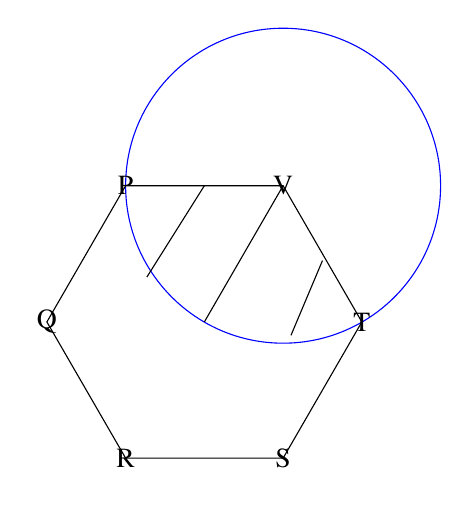
\begin{tikzpicture}
            \draw[blue] (2,3.46) circle (2);
            \draw(1,3.46)--(0.27,2.3);
            \draw(2,3.46)--(1,1.73);
            \draw(2.5,2.509)--(2.1,1.56);
        \draw (0,0) -- (2,0) -- (3,1.73) -- (2,3.46) -- (0,3.46) -- (-1,1.73) -- cycle;
        \node at (0,0) {R};
        \node at (2,0) {S};
        \node at (3,1.73) {T};
        \node at (2,3.46) {V};
        \node at (0,3.46) {P};
        \node at (-1,1.73) {Q};
    \end{tikzpicture}
    \end{center}  
    \end{figure}
    \item An orifice plate is used to measure flow rate of air (density = 1.23 kg/m$^3$) in a duct of 250 mm diameter as shown in figure. The volume flow rate is 1 m$^3$/s. Flow at sections 1 and 3 is uniform and section 2 is located at vena contracta. The diameter ratio, $D_t/D_1$, is 0.66. The flow area at vena contracta, $A_2 = 0.65 A_1$, where $A_t$ is area of the orifice. The pressure difference between locations 2 and 3 in N/m$^2$ is {\underline{\hspace{2cm}}}.
    \begin{figure}[H]
        \centering
        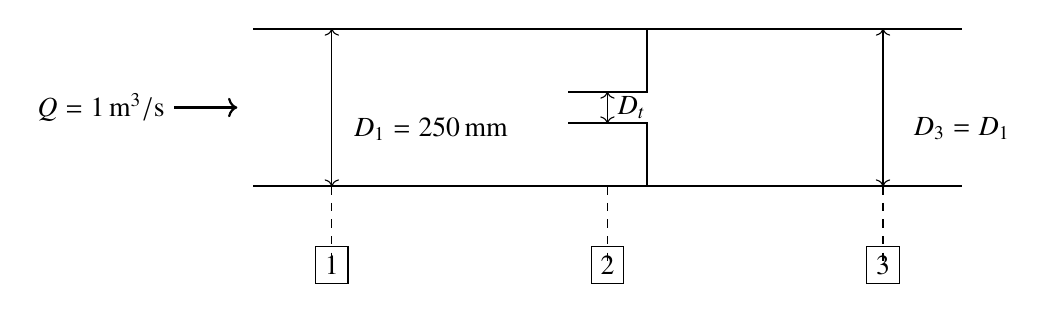
\begin{tikzpicture}
    \draw[thick] (-1, 1) -- (8, 1); 
    \draw[thick] (-1, -1) -- (8, -1); 
    \draw[->, thick] (-2, 0) -- (-1.2, 0);
    \node[left] at (-2, 0) {$Q = 1 \, \mathrm{m^3/s}$};
    \draw[<->] (0, 1) -- (0, -1);
    \node[below] at (1.256, 0) {$D_1 = 250 \, \mathrm{mm}$};
    \draw[thick] (4, -1) --(4, -0.2)--(3,-0.2);
    \draw[thick](4, 1) --(4, 0.2)--(3,0.2);  
    \draw[<->] (3.5, 0.2) -- (3.5, -0.2);
    \node[right] at (3.5, 0) {$D_t$};
    \draw[<->] (7, 1) -- (7, -1);
    \node[below] at (8, 0) {$D_3 = D_1$};
    \node[draw, rectangle] at (0, -2) {1};
    \draw[dashed] (0, -1) -- (0, -2);
    \node[draw, rectangle] at (3.5, -2) {2};
    \draw[dashed] (3.5, -1) -- (3.5, -2);
    \node[draw, rectangle] at (7, -2) {3};
    \draw[dashed] (7, -1) -- (7, -2);
\end{tikzpicture}

 
    \end{figure}
    \item The stress ratio for a completely reversed cyclic loading during a fatigue test is:
        \begin{multicols}{4}
    \begin{enumerate}
        \item $0$
        \item $1$
        \item $-1$
        \item $\frac{-1}{2}$
    \end{enumerate}
    \end{multicols}
    \item Minimum symmetry that a cubic crystal must possess is:
    \begin{enumerate}
        \item Four 3-fold rotation axes
        \item Three 4-fold rotation axes
        \item Three orthogonal mirror planes
        \item Centre of symmetry
    \end{enumerate}
    \item If a material is repelled in an external magnetic field, then it is:
        \begin{multicols}{2}
    \begin{enumerate}
        \item Ferromagnetic
        \item Diamagnetic
        \item Paramagnetic
        \item Antiferromagnetic
    \end{enumerate}
    \end{multicols}
    \item An electron makes a transition from the valence band to the conduction band in an indirect band gap semiconductor. Which one of the following is true?
    \begin{enumerate}
        \item Energy of the electron decreases
        \item A photon is emitted in the process
        \item A phonon is annihilated in the process
        \item A photon is created in the process
    \end{enumerate}
    \item Which one of the following is the characteristic of a screw dislocation?    
    \begin{enumerate}
        \item Dislocation line and Burgers vector are parallel
        \item Direction of motion of dislocation is parallel to the Burgers vector
        \item Atomic displacement due to the movement of the dislocation is in the direction of the motion of the dislocation line
        \item It has a unique slip plane
    \end{enumerate}
    \item The number of vibrational degrees of freedom for a non-linear triatomic molecule are
        \begin{multicols}{4}
    \begin{enumerate}
        \item 9
        \item 6
        \item 4
        \item 3
    \end{enumerate}
    \end{multicols}
    \item An atom is restricted to move in one dimension by making unit jumps either to the left or right,as shown in figure. Assuming that a jump to the left or right is equally probable, the probability of the atom returning back to the starting point after four jumps is
    \begin{figure}[H]
        \centering
        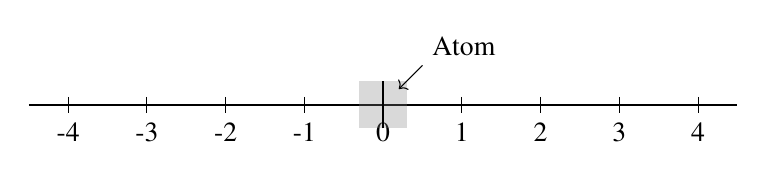
\begin{tikzpicture}
    \draw[thick, -] (-4.5,0) -- (4.5,0);
    \foreach \x in {-4, -3, -2, -1, 0, 1, 2, 3, 4} {
        \draw (\x, 0.1) -- (\x, -0.1);  
        \node[below] at (\x, -0.1) {\x}; 
    }
    \fill[gray, opacity=0.3] (-0.3, -0.3) rectangle (0.3, 0.3);
    \draw[thick] (0, -0.3) -- (0, 0.3);  
    \draw[->] (0.5, 0.5) -- (0.2, 0.2);
    \node[above right] at (0.5, 0.5) {Atom};
\end{tikzpicture}

  
    \end{figure}
    \begin{multicols}{4}
    \begin{enumerate}
        \item 0.250
        \item 0.333
        \item 0.375
        \item 0.500
    \end{enumerate}
    \end{multicols}
    \item For a two-dimensional solid, the variation of lattice specific heat as a function of temperature $T$ (in K, at low temperatures) is given as $C_p = bT^n$, where $b$ is a constant. The value of $n$ is {\underline{\hspace{2cm}}}.
    \item If the cation (C) to anion (A) radius ratio, $\frac{r_C}{r_A}$, is 0.6, then the coordination number (i.e., number of A ions surrounding a C ion) is likely to be {\underline{\hspace{2cm}}}.
\end{enumerate}
\end{document}
